\documentclass[11pt,a4paper]{article}
\usepackage[utf8]{inputenc}
\usepackage[english]{babel}
\usepackage{amsmath}
\usepackage{amsfonts}
\usepackage{amssymb}
\usepackage{makeidx}
\usepackage{graphicx}
\graphicspath{ {./images/} }
\usepackage{cite}
\usepackage{listings}
\usepackage[left=2cm,right=2cm,top=2cm,bottom=2cm]{geometry}
\author{jacmalm@kth.se}
\title{DD2343 Assignment 2}
\begin{document}

\maketitle
\newpage

\section{Dependencies in a Directed Graphical Model}
\subsection{In the graphical model of Figure 1, is $W_{d, n} \perp W_{d,n+1} \mid \theta_{d}, \beta_{1:K}$?}
	Yes.
	
\subsection{In the graphical model of Figure 1, is $ \theta_{d} \perp \theta_{d+1} \mid Z_{d, 1:N}$?}

No.

\subsection{In the graphical model of Figure 1, is $ \theta_{d} \perp \theta_{d+1} \mid \alpha, Z_{1:D, 1:N}$?}

Yes.

\subsection{In the graphical model of Figure 2, is $ W_{d, n} \perp W_{d,n+1} \mid \Lambda_{d}, \beta_{1:K} $?}

No.

\subsection{In the graphical model of Figure 2, is $ \theta_{d} \perp \theta_{d+1} \mid Z_{d, 1:N}, Z_{d+1, 1:N}$?}

No.

\subsection{In the graphical model of Figure 2, is $ \Lambda_{d} \perp \Lambda_{d + 1} \mid \Phi, Z_{1:D, 1:n}$?}

No.

\section{Likelihood of a Tree Graphical Model}

\subsection{Implement a dynamic programming algorithm that for a given $T, \Theta, \beta$ computes $p(\beta \mid T, \Theta)$}

This algorithm is based on the derivation given in video 7.6b, module 7.\\

We start by defining a binary-tree shaped DGM, with root node $A$,  and nodes $B$, $C$ being children of A, and $O_{1}$, $O_{2}$ being both leaves and children of B.

Now, we can define a function $$s(u, i) = p(O \cap\downarrow u \mid u = i) $$

Here $O$ refers to the set of all observations (located on the leaves) and $\downarrow u$ denotes the set of nodes that are descendants of $u$.\\

We know that all nodes (and thus all observations) are descended from the root, thus $s(A, i)$ denotes the probability of all observations, given that the root takes on value $i$. We know that we can get the probability of only the observations from the conditional probability using the product rule and marginalization

$$s(A, i) = p(O \mid A = i)$$
$$p(O \mid A = i) = \frac{p(O, A = i)}{p(A = i)} $$
$$p(O) = \sum_{A} \frac{p(O, A = i)}{p(A = i)}p(A = i)$$
$$p(O) = \sum_{i} s(A, i)p(A=i)$$

Furthermore, we can define a recurrence relationship for $s$, using the conditional independence properties encoded in the DGM
$$s(A, i) = p(O \cap\downarrow B \mid A = i)p(O \cap\downarrow C \mid A = i)$$

"Unmarginalizing" either of these terms results in

$$p(O \cap\downarrow B \mid A = i) = \sum_{j} p(O \cap\downarrow B, B = j \mid A = i)$$

Using the product rule and conditional independence

$$ \sum_{j} p(O \cap\downarrow B, B = j \mid A = i) =  \sum_{j} p(O \cap\downarrow B \mid B = j)p(B = j \mid A = i)$$

Now, we recognize that
$$ p(O \cap\downarrow B \mid B = j) = s(B, j)$$

Putting this together
$$s(A, i) = \sum_{j}s(B, j)p(B = j \mid A = i) \times \sum_{k} s(C, k)p(C = k \mid A = i)$$

We can also see that when we reach node $B$, who has children that are leaves, we reach our base case and the recursion ends.
$$s(B, i) = p(O_{1} \mid B = i)p(O_{2} \mid B = i)$$

Now, in order to calculate $p(O)$, we will need to calculate $s(A, i)$ with $i$ taking on all $K$ values. We also see that as the recursion becomes a layer removed from $A$ we will calculate $s(B, j)$, whose computation does not depend on $i$. Thus we will do the same computations $K$ times. As $s(B, j)$ is itself a recurrent function call with the same problem, these inefficiencies quickly add up. If we instead make use of dynamic programming, and save the result of each $s(u, i)$ that we compute in a map with $(u, i)$ as the key, we will only need to calculate each item once. This makes our algorithm time complexity  $O(Kn)$ where $n= ||nodes||$ as opposed to $K^{d}$ where $d$ is depth of the tree, a great improvement.

Code that implements this algorithm can be found in Appendix 1.

\subsection{Report $p(\beta \mid T, \Theta)$ for each given data}

\subsubsection{Small tree}

	Sample:  0 	Beta:  [nan  2. nan  0.  2.]
	Likelihood:  0.009786075668602368\\

	Sample:  1 	Beta:  [nan  3. nan  0.  0.]
	Likelihood:  0.015371111945909397\\

	Sample:  2 	Beta:  [nan  1. nan  0.  0.]
	Likelihood:  0.02429470256988136\\

	Sample:  3 	Beta:  [nan  0. nan  3.  4.]
	Likelihood:  0.005921848333806081\\

	Sample:  4 	Beta:  [nan  3. nan  3.  3.]
	Likelihood:  0.016186321212555956\\

\subsubsection{Medium tree}

	Sample:  0 \\	Beta:  [nan nan nan nan nan nan nan  1.  3. nan nan nan nan  4. nan nan  1. nan
 nan nan  0. nan nan  3. nan nan  0. nan  0.  4. nan nan  1.  0.  4.  0.
  1.  1. nan  3.  3.  1.  0.  0.  2.  4. nan  1.  2.  3.  0.]\\
	Likelihood:  1.7611947348905713e-18\\

	Sample:  1 \\	Beta:  [nan nan nan nan nan nan nan  0.  0. nan nan nan nan  4. nan nan  3. nan
 nan nan  0. nan nan  3. nan nan  1. nan  3.  1. nan nan  4.  3.  1.  1.
  4.  3. nan  3.  1.  0.  2.  4.  3.  2. nan  4.  4.  0.  0.]\\
	Likelihood:  2.996933026124685e-18\\

	Sample:  2 \\	Beta:  [nan nan nan nan nan nan nan  1.  3. nan nan nan nan  2. nan nan  2. nan
 nan nan  1. nan nan  4. nan nan  4. nan  4.  4. nan nan  2.  1.  2.  3.
  0.  3. nan  3.  2.  2.  2.  1.  4.  2. nan  4.  3.  3.  4.]\\
	Likelihood:  2.891411201505415e-18\\

	Sample:  3\\ 	Beta:  [nan nan nan nan nan nan nan  0.  0. nan nan nan nan  2. nan nan  4. nan
 nan nan  1. nan nan  3. nan nan  2. nan  4.  2. nan nan  4.  4.  2.  3.
  0.  3. nan  3.  4.  1.  2.  3.  4.  2. nan  1.  0.  3.  0.]\\
	Likelihood:  4.6788419411270006e-18\\

	Sample:  4\\ 	Beta:  [nan nan nan nan nan nan nan  4.  1. nan nan nan nan  0. nan nan  1. nan
 nan nan  1. nan nan  0. nan nan  1. nan  0.  1. nan nan  1.  1.  2.  4.
  1.  0. nan  3.  0.  0.  3.  3.  3.  1. nan  2.  3.  3.  1.]\\
	Likelihood:  5.664006737201378e-18\\

\subsubsection{Large tree}

Sample:  0 	\\
	Likelihood:  3.63097513075208e-69

	Sample:  1 	\\
	Likelihood:  3.9405421986921234e-67

	Sample:  2 	\\
	Likelihood:  5.549061147187144e-67

	Sample:  3 	\\
	Likelihood:  9.89990102807915e-67

	Sample:  4\\
	Likelihood:  3.11420969368965e-72

\section{Super Epicentra - Expectation-Maximization}

\subsection{Derive an EM algorithm for the model}

The outline of the expectation maximization algorithm is given in section 9.3 in Pattern Recognition and Machine Learning, by Bishop \cite{book}. The outline is summarized as follows:\\

Given a joint distribution $p(Y, Z \mid \theta)$ the goal is to maximize the likelihood $p(Y \mid \theta)$ w.r.t. $\theta$.
\begin{flushleft}

1.	Choose initial parameters $\theta$\\
2. 	Evaluate $p(Z \mid Y, \theta^{old})$\\
3.	Evaluate $\theta^{new}$ where
$$ \theta^{new} = {arg max}_{\theta} Q(\theta, \theta^{old})$$
and
$$ Q(\theta, \theta^{old}) = \sum_{Z} p(Z \mid Y, \theta^{old})ln(p(Y, Z \mid \theta))$$
4.	Check for convergence, we deem the algorithm to have converged if $p(Y \mid \theta^{new}) - p(Y \mid \theta^{old}) < \varepsilon $. If not converged, repeat from step 2. Otherwise $\theta^{new}$ are our parameter values.

\end{flushleft}

In the outline above, $Y$ denotes the set of observed variables, $Z$ denotes the set of latent variables, and $\theta$ denotes the model parameters. Thus in the context of our model $Y = \lbrace X, S\rbrace$, $Z = \lbrace Z \rbrace$, and $\theta = \lbrace \mu, \tau, \lambda, \pi\rbrace$.

From inspection of the DGM, and taking note of the conditional independence properties encoded by it, we can see that the joint probability distribution of a single data point $n \in N$ is given by:

$$ p(X_{n}, S_{n}, Z_{n} \mid \theta) = \prod_{k} p(Z_{n})p(X_{n} \mid Z_{n})p(S_{n} \mid Z_{n}) $$

Assuming that our data points are sampled independently, the probability of observing the entire dataset, or likelihood, is given by

$$ p(X, S, Z \mid \theta) = \prod_{n} \prod_{k} p(Z)p(X \mid Z)p(S \mid Z) $$
$$ p(X, S, Z \mid \theta) = \prod_{n} \prod_{k} \pi_{k}^{z_{nk}}(N(x_{n} \mid \mu_{k}, \tau_{k}^{-1})P(s_{n} \mid \lambda_{k}))^{z_{nk}} $$

Where $N$ and $P$ denote the Normal and Poisson distribution respectively. The log-likelihood is thus given by
$$ln(p(X, S, Z \mid \theta)) = \sum_{n} \sum_{k} z_{nk}(ln(\pi_{k}) + ln(N(x_{n} \mid \mu_{k}, \tau_{k}^{-1})) + ln(P(s_{n} \mid \lambda_{k})) $$

In practice, a problem arises due to the fact that $Z$ is not observed. This means that we cannot directly use $p(Z \mid Y, \theta^{old})$, but we instead use its expectation w.r.t its posterior distribution. Thus we introduce 

$$\gamma(z_{nk}) = \mathbb{E}(z_{nk}) = \frac{\pi_{k}N(x_{n} \mid \mu_{k}, \tau_{k}^{-1})P(s_{n} \mid \lambda_{k})}{\sum_{j}\pi_{j}N(x_{n} \mid \mu_{j}, \tau_{j}^{-1})P(s_{n} \mid \lambda_{j})}$$

We then want to maximize $$ \mathbb{E_{Z}}(ln(p(X, S, Z \mid \theta)) = \sum_{n} \sum_{k}\gamma(z_{nk})(ln(\pi_{k}) + ln(N(x_{n} \mid \mu_{k}, \tau_{k}^{-1})) + ln(P(s_{n} \mid \lambda_{k}))$$

Comparing this expression with the one given for only a Gaussian mixture model we can see that the difference is given by the added $ln(P(\lambda_{k})$ term. Thus, when we derive the expression with respect to $\mu$ and $\sigma$, this term will disappear. This means that we can use the same solutions for approximating $\mu_{new}, \sigma_{new}$ as given by equations 9.19 and 9.21 in \cite{book}. An analogous argument can be made for the estimation of $\pi$.

Using the same method as in the book for maximizing $\lambda$:


$$ \lambda_{k}^{new} =argmax_{\lambda} \sum_{n} \gamma(z_{nk})(ln(\pi_{k}) + ln(N(x_{n} \mid \mu_{k}, \tau_{k}^{-1})) + ln(P(s_{n} \mid \lambda_{k}))$$

$$ 0 = \frac{\partial}{\partial \lambda_{k}}\sum_{n} \gamma(z_{nk})(ln(\pi_{k}) + ln(N(x_{n} \mid \mu_{k}, \tau_{k}^{-1})) + ln(P(s_{n} \mid \lambda_{k}))$$

$$ 0 = \sum_{n} \gamma(z_{nk})\frac{\partial}{\partial \lambda_{k}}(ln(\pi_{k}) + ln(N(x_{n} \mid \mu_{k}, \tau_{k}^{-1})) + ln(P(s_{n} \mid \lambda_{k}))$$

$$ 0 = \sum_{n} \gamma(z_{nk})\frac{\partial}{\partial \lambda_{k}}ln(P(s_{n} \mid \lambda_{k}))$$

Note that we are able to drop the summation over $k$ due to the fact that if we reverse order of the summation we note that all the $k$ terms are independent equally expressed additions to a quantity we wish to maximize (save for the value of $\lambda_{k}$), and thus we want to maximize all of them independently.\\

The Poisson distribution is defined as
$$ P(\lambda) := f(s_{n}) = \frac{\lambda^{s_{n}}e^{-\lambda}}{s_{n}!} $$
Therefore
$$ln(P(\lambda) = s_{n}ln(\lambda) - \lambda - ln(s_{n}!)$$
and
$$\frac{\partial}{\partial \lambda_{k}}(P(\lambda) = \frac{\partial}{\partial \lambda}(s_{n}ln(\lambda) - \lambda - ln(s_{n}!)$$
$$\frac{\partial}{\partial \lambda}(P(\lambda) = \frac{s_{n}}{\lambda} - 1$$

Plugging this into our derivative of the expected log-likelihood
$$ 0 = \sum_{n} \gamma(z_{nk})(\frac{s_{n}}{\lambda_{k}} - 1)$$
$$ 0 = \sum_{n} (\frac{\gamma(z_{nk})s_{n}}{\lambda_{k}} - \gamma(z_{nk}))$$
$$ \sum_{n}\gamma(z_{nk}) = \sum_{n} \frac{\gamma(z_{nk})s_{n}}{\lambda_{k}} $$
$$ \lambda_{k} =  \frac{\sum_{n}\gamma(z_{nk})s_{n}}{\sum_{n}\gamma(z_{nk})} $$

Observe that this equation is of the same form as the equation for updating $mu$, except that we use $s_{n}$ instead of $x_{n}$.

\subsection{Implement your EM algorithm}

Appendix 2.

\subsection{Apply it to the data provided, give an account of the success and provide visualizations for a couple examples. Repeat it for a few different choices of K.}

I used the directions for plotting the contours of the K different models as provided on the course webpage. Thus I plotted contours for the different Normal distributions, with linewidth signifying the "strength" of the super epicentra,  as given by the Poisson parameter.\\

I superimposed this plot onto a scatter plot of our data points, where the size of the data point is given by that data points $S$ value.\\

I began by fitting the data points with $K = 2$. The models initially looked like this:


\begin{center}
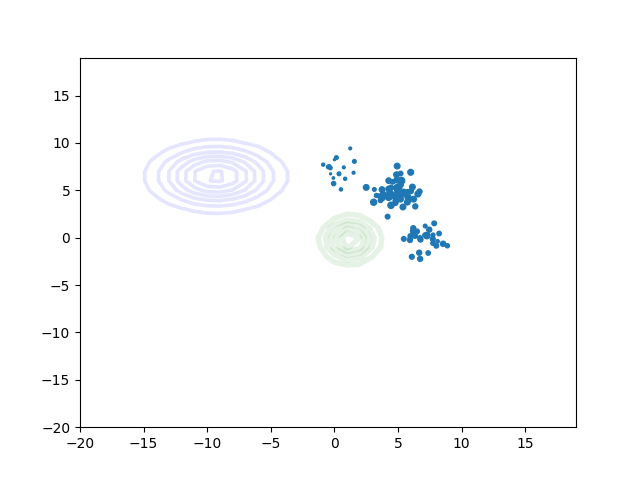
\includegraphics[width=\textwidth]{1_k=2.png}
\end{center}


Optically, we can determine that there are 3 clusters formed by the data points, and as expected our initial clusters do not seem well placed at all.\\

After 1 iteration however,  the clusters are already quite well fitted to the data, with the exception being that the middle cluster is "split" between the two distributions.\\

\begin{center}
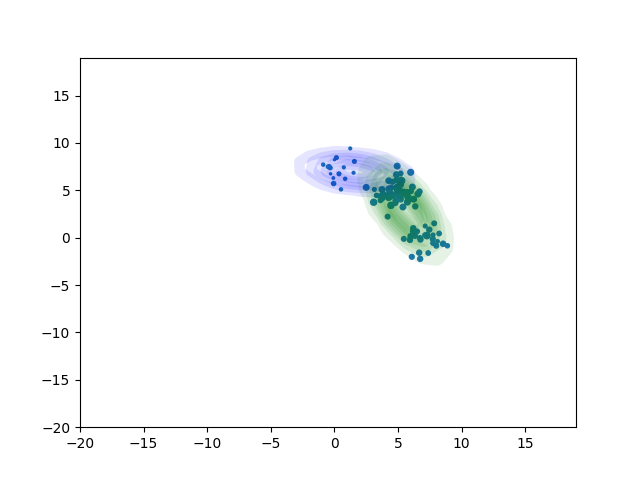
\includegraphics[width=\textwidth]{2_k=2.png}
\end{center}

And by the end, the clusters are about as well fitted as they can be\\

\begin{center}
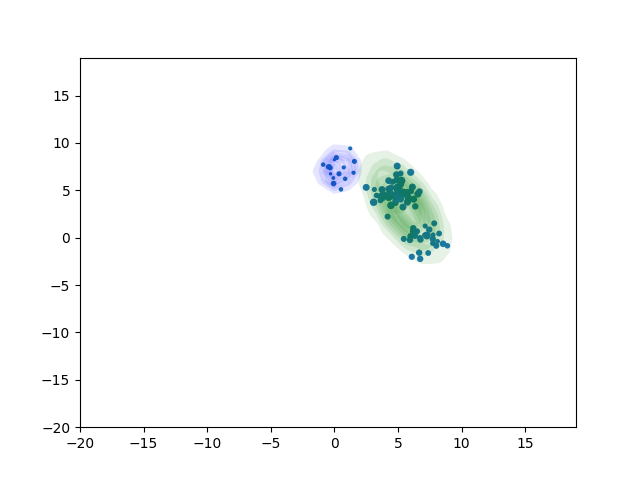
\includegraphics[width=\textwidth]{3_k=2.png}
\end{center}

We can see that the algorithm attempts to make up for the deficiency we have in setting $K=2$ by making the variance of the of the second distribution larger, so that it encompasses both of the clusters not attributed to the first distribution, that also happen to be closer together.\\

If we set $K=3$ and try again, we see quite good results, as expected from our observations of the previous experiment.

\begin{center}
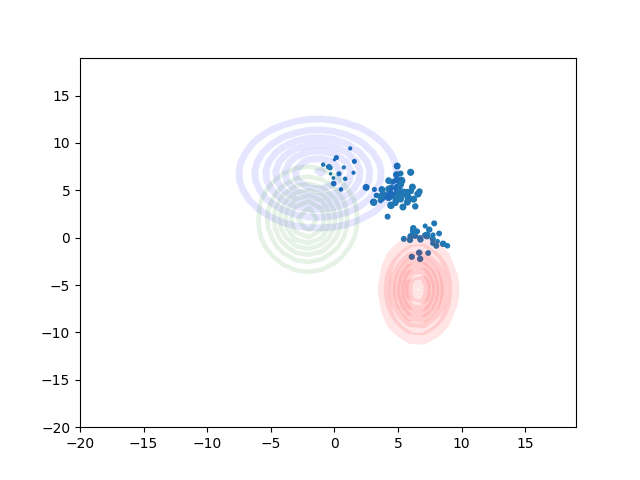
\includegraphics[width=\textwidth]{1_k=3.png}
\end{center}
\begin{center}
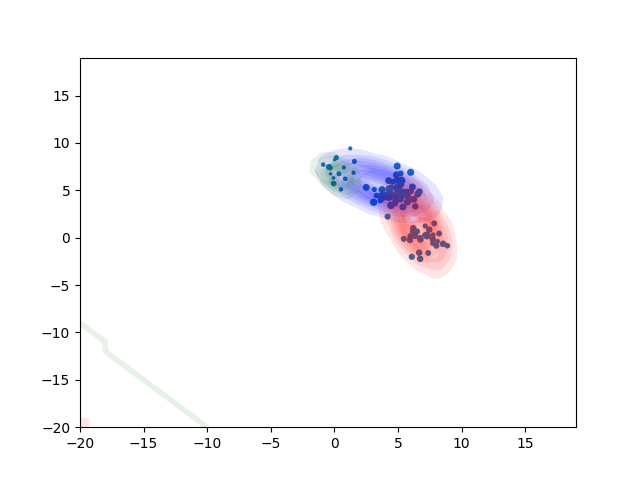
\includegraphics[width=\textwidth]{2_k=3.png}
\end{center}
\begin{center}
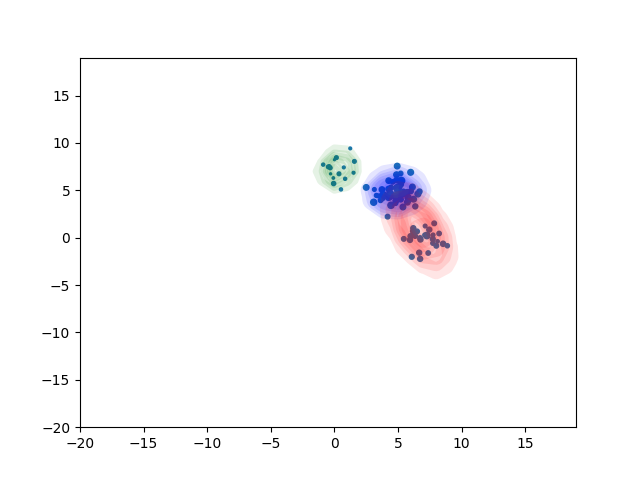
\includegraphics[width=\textwidth]{3_k=3.png}
\end{center}
\begin{center}
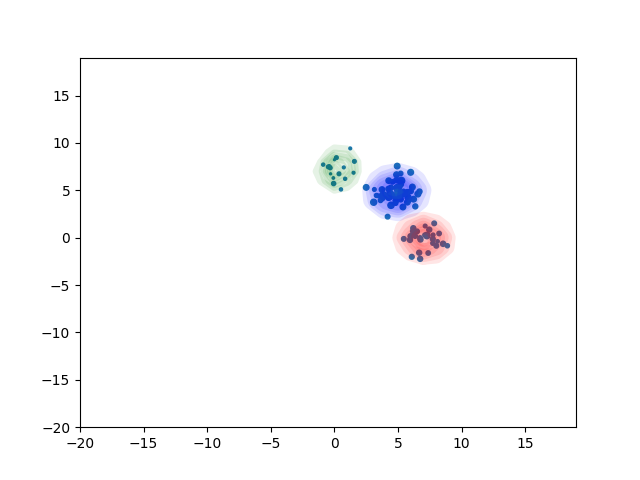
\includegraphics[width=\textwidth]{4_k=3.png}
\end{center}

By the end, the three distributions are well fitted to the three clusters, and the line widths seem correlated to that clusters average size of data points.

An interesting thing happens when we set $K=6$. Of course, there is a lot more chaos, and some distributions end up "sharing" the clusters.

\begin{center}
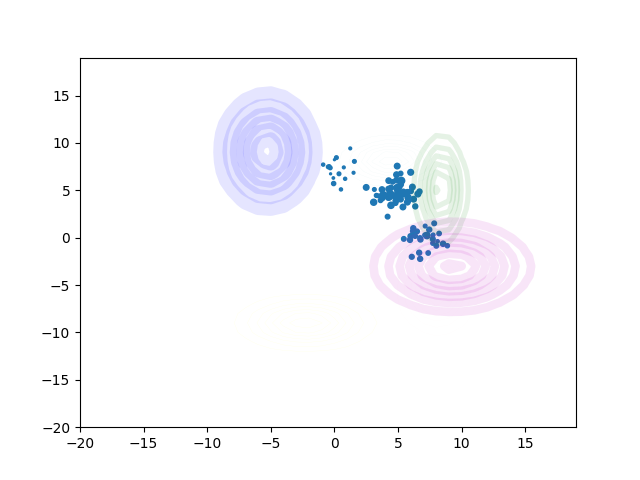
\includegraphics[width=\textwidth]{1_k=6.png}
\end{center}
\begin{center}
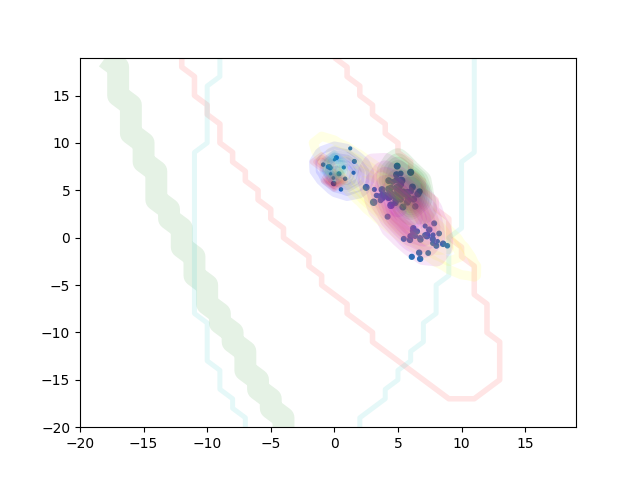
\includegraphics[width=\textwidth]{2_k=6.png}
\end{center}
\begin{center}
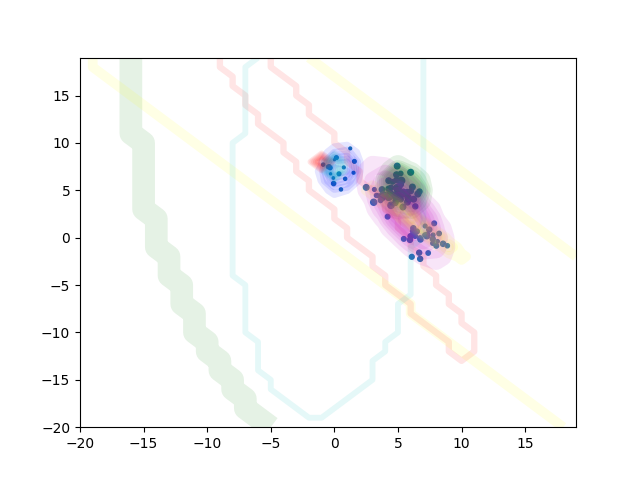
\includegraphics[width=\textwidth]{3_k=6.png}
\end{center}
\begin{center}
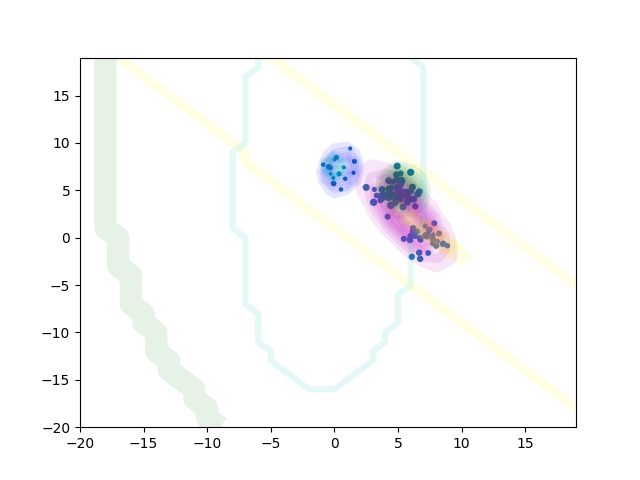
\includegraphics[width=\textwidth]{4_k=6.png}
\end{center}

However, if we look at the difference between the second last and last iteration, we can see that one distribution has disappeared. Also, I noticed that when I ran the code for $K=6$, seemingly randomly I would get an error about not being able to create the Normal distributions with our updated parameters. 

When I began debugging, I noticed that when this would happen, we attempted to instantiate a Normal distribution with certain variance values being equal to zero, and scipy would throw an error. Passing in "allow\textunderscore singular=True" to the constructor of the Normal distribution fixed this. 

This explains why in the images, one distribution disappears. I believe this is caused by the "vanishing variance" problem where if the mean of one cluster is exactly equal to one of the data points, setting its variance to zero contributes an infinite term to our log likelihood calculation, as mentioned in the book \cite{book}.

\section{Appendix}
\subsection{Appendix 1}
\lstinputlisting[language=python]{../code/task_2_2/q2_2.py}

\subsection{Appendix 2}
\lstinputlisting[language=python]{../code/task_2_4/expectation_maximization.py}

\bibliography{citations}
\bibliographystyle{plain}


\end{document}